%!Tex Root = ../main.tex
% ./Packete.tex
% ./Design.tex
% ./Deklarationen.tex
% ./Vorbereitung.tex
% ./Aufgabe1.tex
% ./Aufgabe2.tex
% ./Aufgabe3.tex
% ./Aufgabe4.tex

\section{Appendix}

\begin{frame}[allowframebreaks]{Appendix}{Hinweis zu Hypercubes und Karnaugh Map}
  \begin{itemize}
    \item Wenn sich zwei Knoten nur durch genau $1$ Bit unterscheiden, dann werden sie durch eine Kante verbunden.
  \end{itemize}
  \begin{figure}
      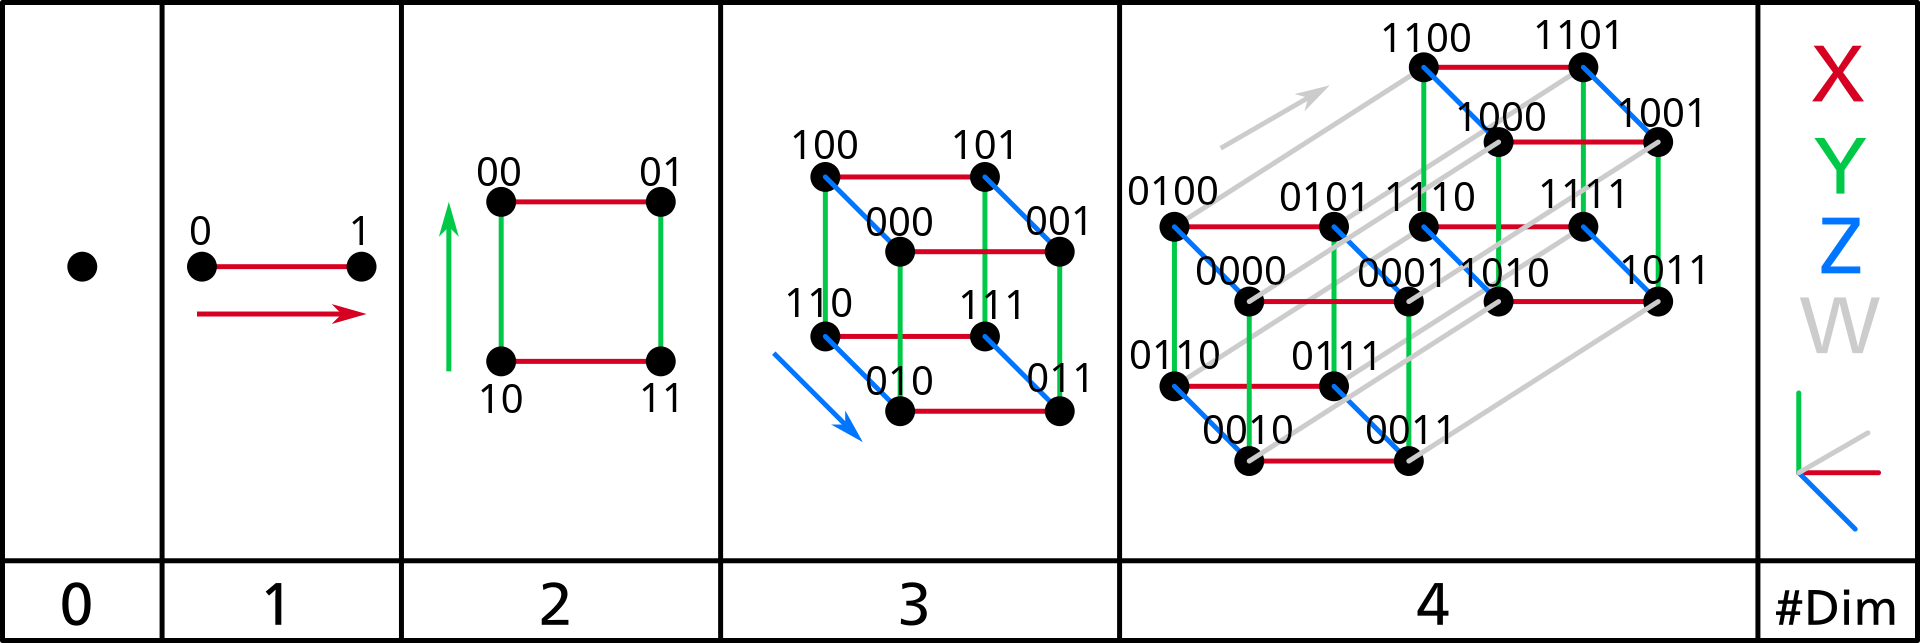
\includegraphics[width=0.8\textwidth, center]{./figures/hypercubes.png}
      \caption{Hypercubes von $n=0$ bis $n=4$}
  \end{figure}
  \newpage
  \begin{figure}
    \centering
    \begin{subfigure}{0.4\textwidth}
       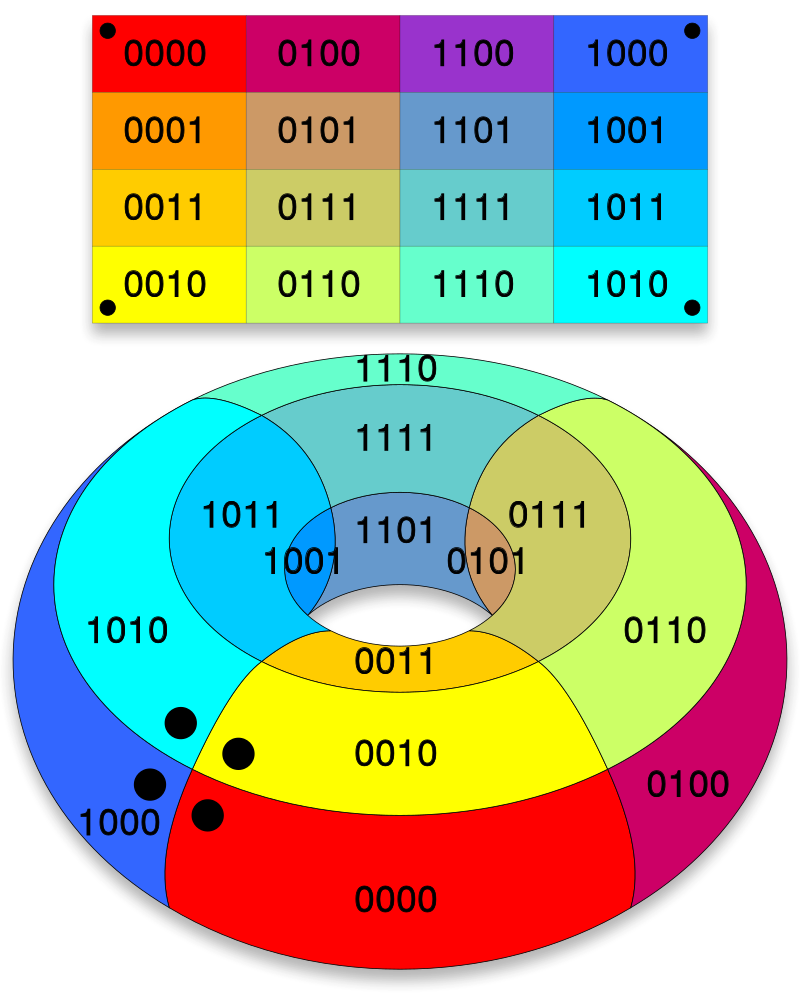
\includegraphics[height=0.4\textheight, center]{./figures/donut.png}
       \caption{Torus oder umgangssprachlich Donut}
    \end{subfigure}
    \begin{subfigure}{0.4\textwidth}
       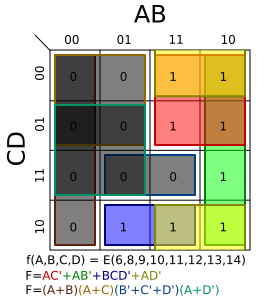
\includegraphics[height=0.4\textheight, center]{./figures/K_map.png}
       \caption{Beispiel für Karnaugh Map}
    \end{subfigure}
  \end{figure}
  \begin{itemize}
      \item Anordnung ist so, weil man einen Hypercube bis $n=4$ (Tesseract) in einer flachen Tabelle darstellen will und im Hypercube gibt es immer nur eine Kante, wenn es nur genau $1$ Bit Unterschied bei $2$ Knoten gibt.
      \item In der Karnaugh Map sind entsprechend immer nur Bitvektoren benachbart, die sich nur in einem Bit unterscheiden. 
      \item Wie bei einem Donut sind Reihen und Spalten miteinander von unten nach oben und von links nach rechts über die Tabelle hinausgehend benachbart.
      \item Von $\overline{a}b$ zu $ab$ gibt es nur $1$ Änderung. Von $\overline{a}b$ zu $a\overline{b}$ gibt es dagegen $2$ Änderungen. Daher sind $\overline{a}b$ und $ab$ benachbart.
  \end{itemize} 
\end{frame}
 

\begin{frame}[allowframebreaks]{Appendix}{Kurzschluss}
  \begin{columns}
    \begin{column}{0.5\textwidth}
      \begin{itemize}
        \item $I=\dfrac{U}{R}$
        \item $P = U\cdot I$
      \end{itemize}
    \end{column}
    \begin{column}{0.5\textwidth}
      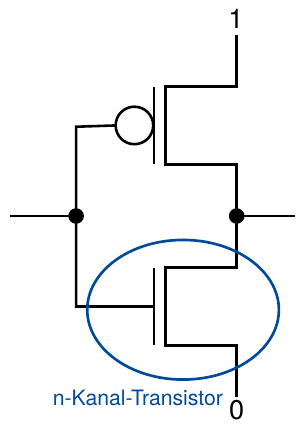
\includegraphics[height=0.6\textheight]{./figures/inverter.png}
    \end{column}
  \end{columns}
\end{frame}

\begin{frame}{Appendix}{Transistoren}
  \begin{itemize}
    \item Ströme steuern. Man kann den Stromfluss innerhalb einer elektrischen Schaltung abbremsen, sodass überhaupt kein Strom fließt (der Transistor funktioniert als Schalter). Man kann aber den Stromfluss auch stark beschleunigen, wodurch ein viel stärkerer Strom fließt (der Transistor funktioniert als Verstärker).
    \item im Kern ist ein Transistor entweder ein strom- oder spannungsgesteuerter Widerstand. Feldeffekttransistoren sind spannungsgesteuerte, Bipolartransistoren sind stromgesteuerte Widerstände.
    \item Unterschiede bei Art der \alert{Lagungsträger}, die zum Stromfluss beiträgt. Bei einem \alert{Bipolartransistor} sind das Elektronen und Löcher. Daher kommt auch der Teil \enquote{Bi} im Namen. Bei einem \alert{Feldeffekttransistor} sind das hingegen entweder Elektronen oder Löcher, also nur eine Art an Ladungsträger.
    \item Feldeffekttransistoren werden überwiegend überall dort verwendet, wo hohe Ströme , Bipolartransistoren hingegen dort, wo geringe Ströme fließen.
  \end{itemize}
\end{frame}

\begin{frame}[allowframebreaks]{Appendix}{Bipolartransistoren}
	\begin{figure}
    \begin{subfigure}{0.4\textwidth}
      \centering
      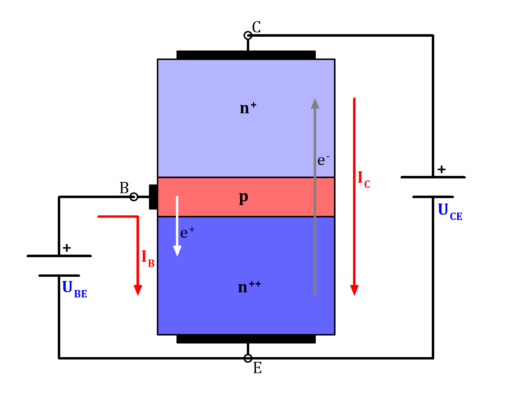
\includegraphics[height=0.5\textheight]{figures/pnp-Transistor}
      \caption{PNP-Transistor}
      \label{fig:pnp-transistor}
    \end{subfigure}
    \begin{subfigure}{0.4\textwidth}
      \centering
      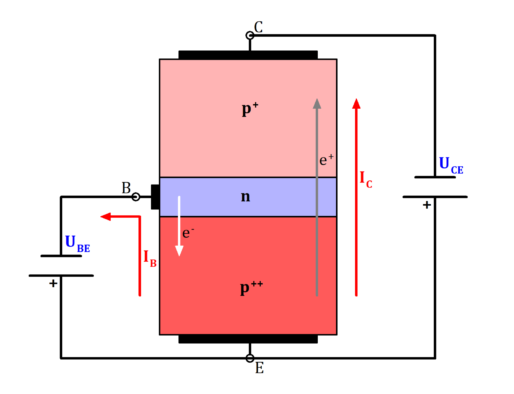
\includegraphics[height=0.5\textheight]{figures/npn-Transistor}
      \caption{npn-Transistor}
      \label{fig:npn-transistor}
    \end{subfigure}
	\end{figure}
  \begin{itemize}
    \item \alert{drei Anschlüsse:} Collector (C), Base (B) und Emitter (E)
  \end{itemize}
\end{frame}

\begin{frame}[allowframebreaks]{Appendix}{Feldeffekttransistoren}
  \begin{figure}
    % \begin{subfigure}{0.4\textwidth}
      \centering
      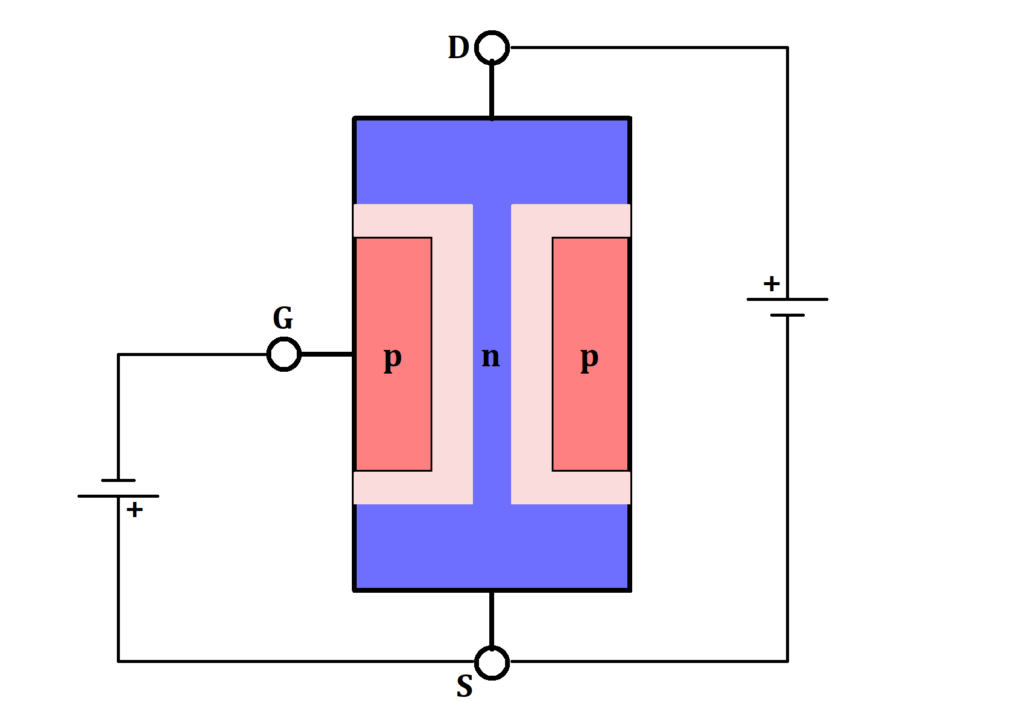
\includegraphics[height=0.5\textheight]{figures/n-Kanal-Feldeffekttransistor.png}
      \caption{n-Kanal-Feldeffekttransistor}
    % \end{subfigure}
    % \begin{subfigure}{0.4\textwidth}
    %   \centering
    %   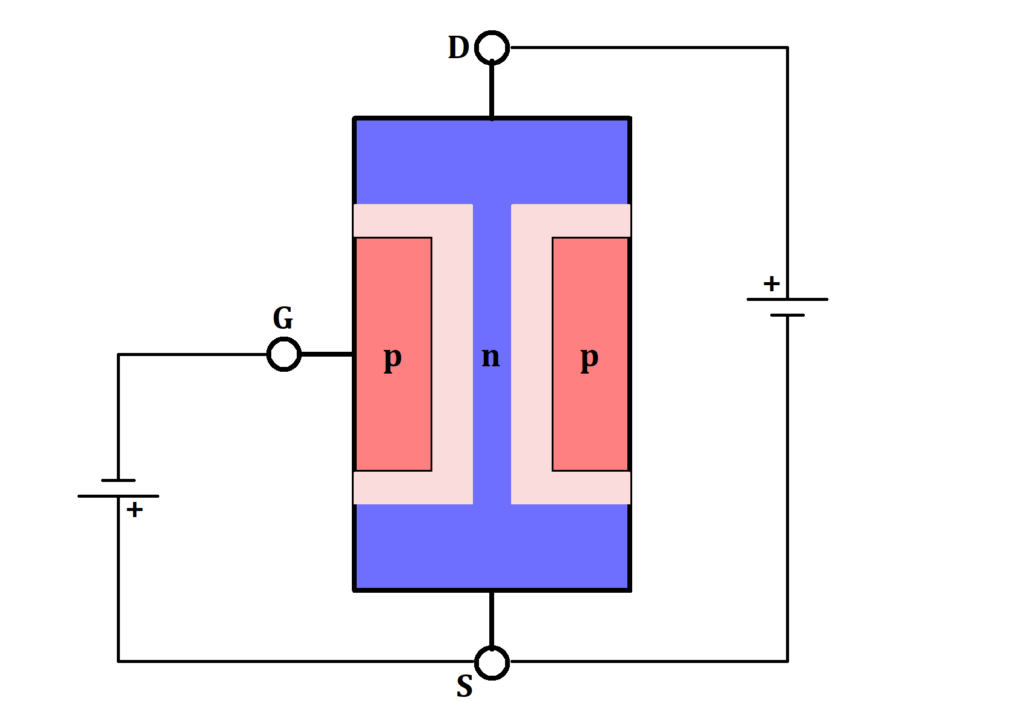
\includegraphics[height=0.5\textheight]{figures/n-Kanal-Feldeffekttransistor.png}
    %   \caption{p-Kanal-Feldeffekttransistor}
    % \end{subfigure}
  \end{figure}
  \begin{itemize}
    \item \alert{drei Anschlüsse:} Drain (D, \enquote{Senke, Abfluss}), Gate (G, \enquote{Tor}) und Source (S, \enquote{Quelle, Zufluss})
    \item Sperrschicht-Feldeffekttransistor (SFET, engl. JFET)
    \item Je nachdem wie der Kanal, durch denen die Ladungsträger fließen, dotiert ist, findest man die Bezeichnungen n-Kanal-FFET und p-Kanal-FFET
  \end{itemize}
\end{frame}

% % Beweis Euklidischer Algorithmus
% diese allgemeine mit Wertigkeit usw.
% Wie N- und P-Kanal-Transistoren funktionieren
% Polynomring
% Übersicht Implikation
% Methematische Logik, a und ~a, a oder ~a
% Necessary and Sufficient, Beiespiel mit Kurvenkdiskussion
% Modelle, Strukturen, Quantoren Bild
% RETI ist eine Register-Memory Architektur, Accumulator Architektur
% es gibt Kontrollsignale und die anderen Signale
% wie Hypercubes genau funktionieren

% Emails werden noch beantwortet
% in welcher Reihenfolge am sinnvollsten bearbeiten?
% Klarstellung Begriff Boolesche Algebra
% surjektiv bezüglich Bildmenge ist sowieso klar, deswegen spricht man es nicht aus, aber ja stimmt
% wie sich das Binärsystem für Kommastellen fortsetzt mit 2^{-1}
% bei KNF und Karnaugh Map muss man immer von der negierten Maxtermen ausgehen bei eintragen in die Tabelle. Wobei es einfach ausgedrückt einfach die Invertierung der anderen Tabelle ist
% wie man sich P-Kanal und N-Kanal gut merken kann, p und 0, N und I und lässt genau dann durch, wenn es 0 ist
% die Sache mit 11111 möglichst große Zahl
